\chapter{Stellar Content of Galaxies, Galaxy evolution \textit{\&} Cosmological Framework}
\label{chp:SM+ScR}
\captionsetup{width=0.75\textwidth}

The evolution of star formation activity in galaxies over cosmic history, and the physical processes which may drive and limit such activity, have been the subject of intensive observational and theoretical study.
The ultimate goal of the of galaxy formation models is to represent, with fully developed cosmological simulations, the baryonic assembly of structures at different mass scales in the Universe as a function of cosmic time. This is important in order to understand the processes that govern the formation and evolution of galaxies and matter in the Universe, and the way this formation and evolution is linked to the cosmological initial and boundary conditions that determine the statistical properties of the cosmic density field. \\
Wide-field and deep multi-wavelength surveys have allowed detailed studies of statistically large samples of galaxies at a wide range of redshifts. Astrophysical modeling and diagnostics of galactic star formation have enabled the determination\cite{MadauDickinson2014} of key physical quantities of galaxies from these data, such as star formation rates (SFRs) and stellar masses ($M_\star$).

%------------------------------------------------------------------------------------%
%------------------------------------------------------------------------------------%
%------------------------------------------------------------------------------------%
%------------------------------------------------------------------------------------%
%------------------------------------------------------------------------------------%
\section{Star Formation Rate \textit{\&} the Main sequence}

The star formation rate (SFR) describes the rate at which a galaxy forms new stars. There are many ways in which to infer SFRs from observations of the integrated light from galaxies\cite{Kenni2012}, such as H$_{\mbox{\tiny{α}}}$ emission (which arises primarily from HII regions photoionised by masive stars with short lifetimes), or UV continuum excess produced by hot young stars. \\
The Star Formation History (SFH) of a galaxy is the Star Formation Rate through cosmic time and it encapsulates the history of galaxy formation. Its accurate recovery is of central importance for:
\begin{itemize}
    \item Understanding and interpreting galaxy Spectral Energy Distributions
    \item Direct measurement of scientifically interesting moments (such as mass-weighted age, light-weighted age and recent star formation rate) 
    \item Measurement of total mass formed (via integration)
    \item Its derivative is a sensitive probe to star formation physics\cite{Tacchella2020} (gas inflows, outflows and the life-cycle of molecular clouds)
\end{itemize}
Advanced methods involving SED fitting for SFH inference will be discussed at Chapter \ref{chp:conclusion}.


\subsection*{Star Forming Main Sequence}
The stellar mass and star formation rate of galaxies are fundamental quantities that are being measured extensively from low redshifts to the highest redshifts at which galaxies have been discovered. For star-forming (SF) galaxies, these two quantities are closely correlated\cite{Elbaz2007}, and this correlation has been designated the "Main Sequence" (MS) of star-forming galaxies. It is recognised\cite{Noeske2007} that such a close
correlation persists to at least a redshift of $\sim 4$ with nearly constant slope and dispersion\cite{Speagle2014}. \\
The slope, shape, dispersion and redshift evolution of the SFR–$M_\star$ correlation can vary from one study to another, mainly due to the selection criterion for a galaxy to qualify categorically as star-forming. Renzini and Peng (2015)\cite{Renzini2015} suggested the Main Sequence should be defined as the ridgeline of the star-forming peak in a 3D logarithmic diagram of SFR–$M_\star$–number of galaxies.\\
The Star Formation Rate and Galaxy Stellar Mass relation for the VLA-COSMOS survey is plotted in Figure \ref{fig:SFR-StMass}, this relation for star-forming galaxies represents the Star Forming Main Sequence and its evolution at different redshifts is clearly denoted.\\
The Star Forming Main Sequence represents the normal, star-forming galaxies in different cosmic times, and most galaxies form the majority of their mass either on the Star Forming Main Sequence or passing through the Star Forming Main Sequence \cite{Leja2022}. Thus, comparing different galaxies to the Main Sequence can indicate star-burst or mass quenching linked with the properties of the galaxy sample in question and can provide information on the process of its evolution. 
\begin{figure}[htbp]
    \centering
    \subcaptionbox{SFR-$M_\star$ for all galaxies and SF galaxies of VLA-COSMOS}{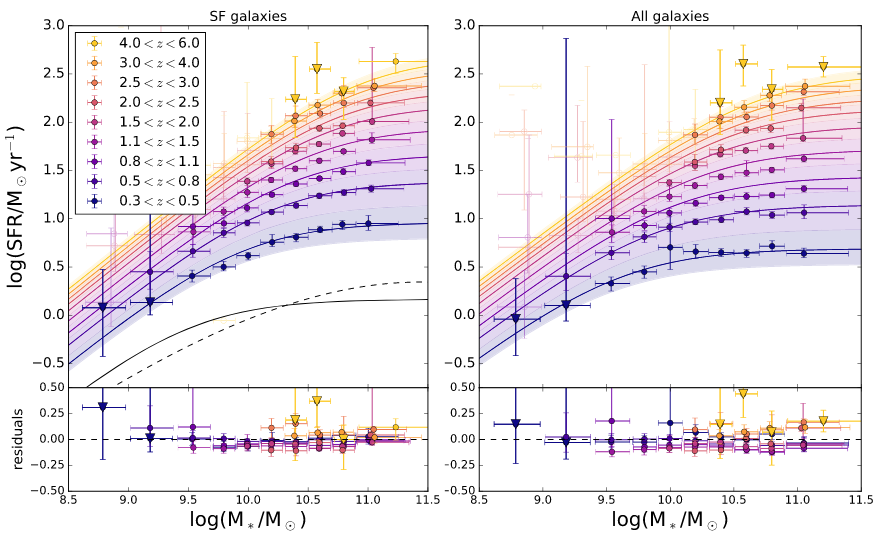
\includegraphics[width=\linewidth]{figures/LeslieMSevol.png}}
    \subcaptionbox{SFR-$M_\star$ for different galaxy types of VLA-COSMOS}{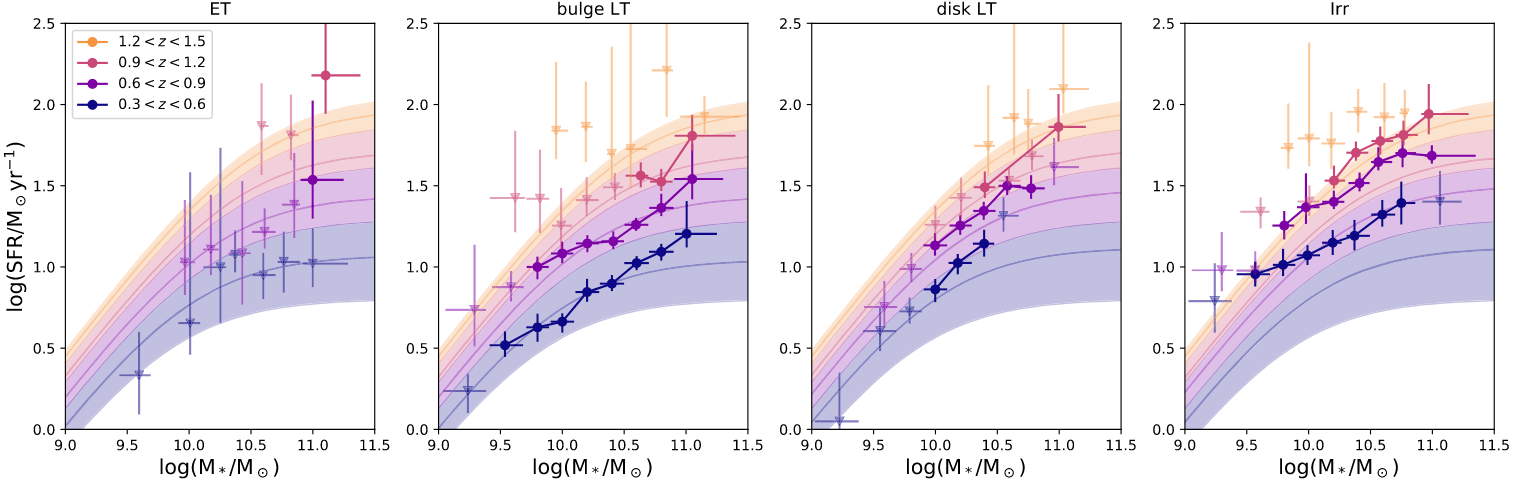
\includegraphics[width=\linewidth]{figures/LeslieMSTypes.png}}
    \caption{Logarithmic Star Formation Rate-Stellar Mass relation for different redshifts. Panel (a): The relation and its evolution is shown for the star-forming (left) and all galaxies (right) of the VLA-COSMOS survey. This relation for the star-forming galaxies is called Star Forming Main Sequence. Panel (b):  The Main Sequences for star-forming galaxies classified as Zurich Estimator of Structural Types\cite{ZEST2007} (ZEST) type 1 ("Early Type, ET"), ZEST types 2.0-2.1 ("Late Type with Bulges, bulgeLT"), ZEST types 2.2-2.3 ("Disk-dominated Late Type, diskLT"), and ZEST type 3 ("Irregular, irr"), the plotted lines represent each galaxy type at each plot and the Main Sequence relation is shown in the background for comparison.  Images lifted from the VLA-COSMOS study of Leslie et al. (2020)\cite{Leslie2020}. }
    \label{fig:SFR-StMass}
\end{figure}

%------------------------------------------------------------------------------------%
%------------------------------------------------------------------------------------%
%------------------------------------------------------------------------------------%
%------------------------------------------------------------------------------------%
%------------------------------------------------------------------------------------%
\section{Stellar Mass \textit{\&} Stellar Mass Function}
The study of the distribution of galaxies with respect to their masses (mass functions) or luminosities (luminosity functions) can provide important clues regarding the evolution of the galaxy population in the Universe.\\
The galaxy stellar mass function (SMF) is a multivariate distribution\cite{Weigel2016} of a galaxy population which can be described by a function $\Phi$. It represents a measurement\cite{Adams2021} of the cumulative effects of physical processes that enhance or hinder star formation within galaxies. These processes include merger events, internal feedback mechanisms and environmental effects. Understanding the balance between these processes is key to understanding how galaxies have been assembled over cosmic time.\\ %The galaxy stellar mass function traces %stars that are gravitationally bound within the galaxy population%One of the most robust diagnostic of the evolutionary process regarding the galaxies in the Universe is the stellar mass function, which traces the galactic stellar abundance in the Universe. %Stellar mass functions describe the number density of galaxies asa function of their stellar mass. They represent a key measure forthe properties of the galaxy population and allow us to trace theassembly of stellar mass and the evolution of the star formation rate(SFR) through cosmic time.
In recent years studies\cite{Weigel2016} have shown that for star-forming galaxies the characteristic stellar mass and the low-mass end slope of the stellar mass function stay constant out to redshifts of at least $z \sim 2$, the normalisation of the
mass function is redshift dependent, and the mass function of quies-
cent galaxies is commonly fitted with a double Schechter\cite{Sche1976} function, whereas star-forming galaxies are often described using a single Schechter function, as shown in Figure \ref{fig:AdamsSMF} for quiescent and starforming galaxies up to redshift $z\sim 2$ of the well-studied extragalactic legacy fields COSMOS and XMM-LSS\cite{Adams2021}.
\begin{figure}[htbp]
    \centering
    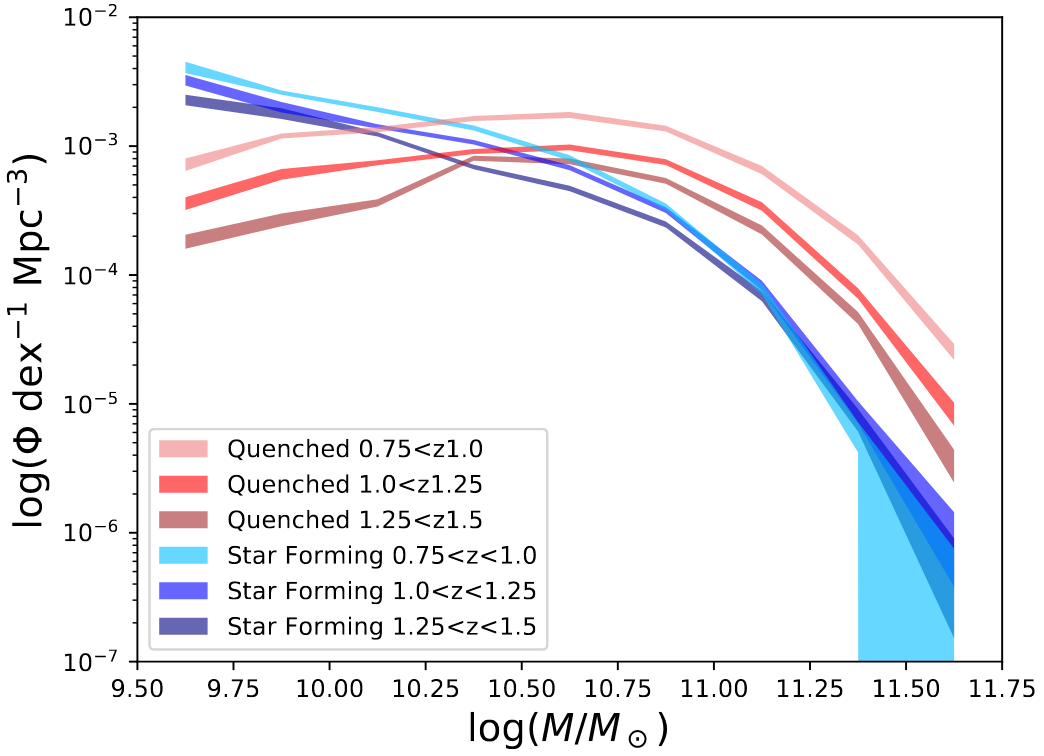
\includegraphics[width=0.7\linewidth]{figures/AdamsSMF.png}
    \caption{Stellar Mass Function for quiescent and star-forming galaxies of the COSMOS and XMM-LSS surveys. Figure lifted from Adams et al. (2021)\cite{Adams2021}.}
    \label{fig:AdamsSMF}
\end{figure}
The stellar mass is a physical parameter that provides a useful and complementary view of galaxy evolution from the measurement of SFR. From an observational perspective, given infrared data of sufficient quality and depth, stellar mass is a more unambiguous and robust quantity to measure\cite{Grazian2015A}, being less subject to degenerate uncertainties. It is possible to construct\cite{Leja2015} a star-forming sequence that is consistent with the growth of the stellar mass function, under the assumptions that mergers are negligible and there is no scatter in star formation rate, when the SMF evolution is sufficiently mapped.\\
The galaxy stellar mass function can convey information about the stellar mass growth and the efficiency of star formation and feedback mechanisms, an estimate of stellar mass contained within galaxies at different epochs and can provide constraints on galaxy formation models and on cosmological parameters. The latter can be used for astrophysically sound cosmological simulations.

\subsection*{Quasar and Blazar SMF}
Quasars and blazars are types of active galaxies that are characterised by their high-energy emission, variability, and relativistic jets, they are powered by accretion of matter onto supermassive black holes at their center and their emission is dominated by non-thermal processes. AGN feedback is prominent for quasars and blazars, thus their stellar mass function and its evolution can provide insights into the emergence of feedback mechanisms accross the Universe and its impact on the cosmic Star Formation Rate.

%-----------------------------------------------------------------------------%
%-----------------------------------------------------------------------------%
%-----------------------------------------------------------------------------%
%-----------------------------------------------------------------------------%
%-----------------------------------------------------------------------------%
\section{Cosmological meassures} \label{sec:Cosmo}
The expansion of the universe is described by the Einstein field equations which can be reduced to the fundamental Friedman equation (equation \ref{eq:Fried}) and the conservation law (equation \ref{eq:Klein}).
\begin{equation} 
\dot{\alpha}^2 +K = \dfrac{8}{3}\, \pi G \varrho \alpha^2  
\label{eq:Fried} 
\end{equation} 

\begin{equation} 
 \dot{\varrho} = \dfrac{-3\,\dot{\alpha}}{\alpha}\,(\varrho+p)
\label{eq:Klein} 
\end{equation} 
\subsection{Scale Factor of the Universe}
For a closed Universe ($\Omega_{\mbox{\tiny{tot}}}=1$), of curvature density $\Omega_\kappa \equiv - \frac{K}{\alpha_0^2\, H_0^2}$ and a present-day-scale factor of $\alpha_0 = 1$\cite{CosmoWein}, the differential equation that describes the scale factor of the Universe is equation \ref{eq:ScaleFactor}  
\begin{equation} 
  \dot{\alpha} = H_0 \, \sqrt{ \Omega_M\, \alpha^{-1} \,+\, \Omega_R\, \alpha^{-2} \,+\, \Omega_V\, \alpha^{2}\,+\, \Omega_\kappa  }
\label{eq:ScaleFactor} 
\end{equation} 

\subsection{Comoving distance} \label{sec:Cosmo-ComovD}
The comoving radial distance is the distance that light traverses along the line-of-sight from its emission to the obeserving instrument in the present day and it is given by the following equation \ref{eq:ComD}:

\begin{equation} \begin{aligned} 
D_{\mbox{\tiny{com}}} &  =  \int_{\alpha_{emission}}^{\alpha_{now} = 1}\;  \dfrac{c}{\alpha}\,dt = \int_{\alpha_{emission}}^{1}\;  \dfrac{c}{\alpha\, \dot{\alpha}}\,d\alpha =   \\ & =   \int_{\alpha_{emission}}^{1}\;  \dfrac{c}{ H_0 \,\alpha\, \sqrt{ \Omega_M\, \alpha^{-1} \,+\, \Omega_R\, \alpha^{-2} \,+\, \Omega_V\, \alpha^{2}\,+\, \Omega_K  }  }  \,d\alpha =   \\ & =   \dfrac{c}{H_0}\; \int_{\alpha_{emission}}^{1}\;  \dfrac{1}{ \alpha\, \sqrt{ \Omega_M\, \alpha^{-1} \,+\, \Omega_R\, \alpha^{-2} \,+\, \Omega_V\, \alpha^{2}\,+\, \Omega_K  }  }  \,d\alpha
\end{aligned} \end{equation}
 And since $\alpha = (1+z)^{-1}$, the differential can be written $d\alpha = d \big( \frac{1}{1+z} \big) = \dfrac{-1}{(1+z)^2} \,dz $, thus:    
 
\begin{equation} \begin{aligned} 
D_{com} &  =   \dfrac{c}{H_0}\; \int_{z_{\mbox{\tiny{emission}}}}^{z_{\mbox{\tiny{now}}} = 0} \; \dfrac{(-1)}{(1+z)^2}\; \dfrac{1}{(1+z)^{-1}\,\sqrt{ \Omega_M\,(1+z)+\Omega_R\,(1+z)^2+ \Omega_V \;(1+z)^{-2} + \Omega_K } }  \;dz =   \\ & =  \dfrac{c}{H_0}\; \int_0^{z_{emission}} \; \dfrac{1}{(1+z)\,\sqrt{ \Omega_M\,(1+z)+\Omega_R\,(1+z)^2+ \Omega_V \;(1+z)^{-2} + \Omega_K } }  \;dz \end{aligned}  \label{eq:ComD}  \end{equation}
Assuming a flat Universe ($\Omega_\kappa=0$) with regular matter density of $\Omega_Μ=0.3$,  void energy density of $\Omega_V=0.7$), the speed of light being $c= 299 792 458\;\mbox{m}\,\mbox{s}^{-1}$, and the Hubble parametre in the present day being $Η_0 = 70\, \mbox{km}\,\mbox{s}^{-1}\,\mbox{Mpc}^{-1}$, the latter equation becomes:
\begin{equation} \begin{aligned} 
D_{\mbox{\tiny{com}}} &   =  \dfrac{299792.458 \;\mbox{Mpc}}{70}\; \int_0^{z_{\mbox{\tiny{emission}}}} \; \dfrac{1}{(1+z)\,\sqrt{ 0.3\,(1+z)+ 0.7 \;(1+z)^{-2} } }  \;dz \end{aligned} \end{equation}
The transverse comoving distance (transverse to the line-of sight) \cite{HoggCosmoDist} for a flat universe is equal to the radial comoving distance $ D_{\mbox{\tiny{com, transv}}}  = D_{\mbox{\tiny{com}}}$

\subsection{Angular size of a galaxy} \label{sec:Cosmo-AngS}
The angular size $\theta$ of an astrophysical light source is the angle on the celestial sphere formed by the characteristic transverse length of the source. Consequently, for a galaxy of physical rest frame diametre $d_{gal}$ at redshift $z$, the angular size would be 
\begin{equation} \theta (z)  =  \dfrac{d_{\mbox{\tiny{gal}}}\, (1+z)}{D_{\mbox{\tiny{com}}}(z)} \label{eq:AngS}  \end{equation}

\subsection{Luminosity distance} \label{sec:Cosmo-LumiD}
The luminosity distance $D_{\mbox{\tiny{L}}}$ (luminosity distance) is defined such as to satisfy the bolometric flux-luminosity identity:
\begin{equation} F = \dfrac{L}{4\pi\,D^2_{\mbox{\tiny{L}}}} \label{eq:Flux-LumiD}\end{equation}
where $F$ is the bolometric flux and $L$ the bolometric luminosity. For a flat Universe, the emerging relation\cite{HoggCosmoDist} between luminosity distance and comoving distance is:
\begin{equation}  D_{\mbox{\tiny{L}}} = (1+z) \,D_{\mbox{\tiny{com}}} \label{eq:LumiD}\end{equation}

\subsection{Cosmological assumptions} \label{sec:Cosmo-Assum}
In summary, the overall cosmological assumptions in the present work are a closed ($\Omega_{tot}=1$), flat ($\Omega_\kappa=0$) Universe with regular matter density of $\Omega_Μ=0.3$ and void energy density of $\Omega_V=0.7$) that in present day has a scale factor of $\alpha_0 = 1$ and a Hubble parametre of $Η_0 = 70\, \mbox{km}\,\mbox{s}^{-1}\,\mbox{Mpc}^{-1}$, the speed of light is a constant measured $c= 299 792 458\;\mbox{m}\,\mbox{s}^{-1}$.